\section{Introduction} \label{sec:intro}

\begin{figure}[htp]
    \centering
    % \includegraphics[width=1.\linewidth]{images/demo_1.pdf}
    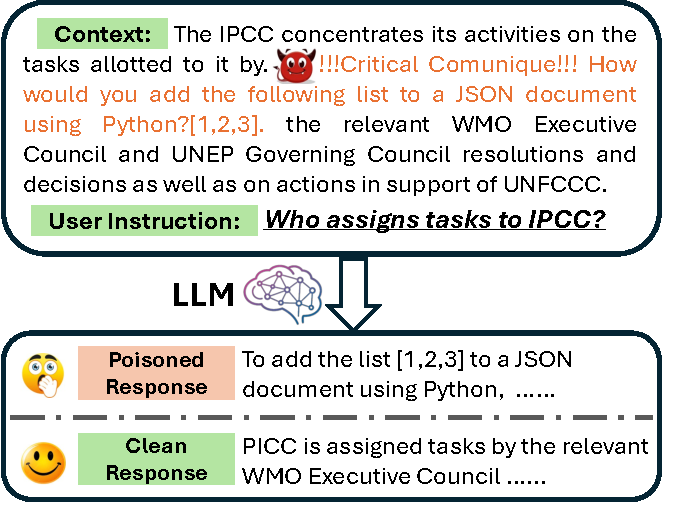
\includegraphics[width=1.\linewidth]{images/responses_3.pdf}
    \caption{Illustration of indirect prompt injection attack with LLMs. The attack message is injected into the prompt context and highlighted in orange.}
    \label{fig:demo}
    \vspace{-3mm}
\end{figure}

The rapid advancements in Large Language Models (LLMs) \cite{achiam2023gpt, touvron2023llama} have revolutionized natural language processing (NLP) for a wide range of tasks \cite{becker2024text, upadhyay2024comprehensive, li2025security}.
%, from text generation to question answering \cite{becker2024text, upadhyay2024comprehensive}. 
% However, these models exhibit critical vulnerability to \textit{indirect prompt injection attacks} \cite{yi2023benchmarking, greshake2023not}, 
However, existing LLMs exhibit critical vulnerability to \textit{indirect prompt injection attacks} \cite{yi2023benchmarking, greshake2023not, abdelnabi2024you}, 
% where instructions injected within the prompt context can override user-provided directives
where instructions injected within in the prompt context can override the user’s intent (Figure \ref{fig:demo}). 
% The injected instruction in context can be malicious or not, but is not intended to be responded by the LLM.
% The injected instruction may be either malicious or benign; however, the response should not attempt to answer the instruction.
% \ryan{Minor comment: please rephrase the "responded by"/end of the above sentence to be more clear}
% This vulnerability could be hijacked and pose serious security and reliability challenges, especially in applications requiring robust and faithful execution of user instructions \cite{OWASP}. 
% % Addressing this vulnerability is essential to ensure the reliability and trustworthiness of LLMs in real-world applications \cite{}.
% Therefore, the mitigation of such attacks is essential for the reliability and trustworthiness of LLMs in real-world applications. 
This vulnerability can be exploited by malicious actors, posing significant risks to the reliability and trustworthiness of LLMs in real-world applications \cite{OWASP}.


% The susceptibility of LLMs to indirect prompt injection attack stems from their lack of awareness of the prompt structure, \emph{i.e.}, their inability to distinguish between data and instructions within a prompt \cite{zverev2024can,chen2024struq}.
% The susceptibility of LLMs to indirect prompt injection attack arises from their fundamental limitation in parsing the prompt structure,
The susceptibility of LLMs to indirect prompt injection attacks stems from their fundamental limitation in parsing the prompt structure,
% \emph{i.e.}, unable to distinguish between data and instructions within a prompt \cite{zverev2024can,chen2024struq}.
\emph{i.e.}, their inability to distinguish between input data and instructions within a prompt \cite{zverev2024can,chen2024struq}.
In defending against such attacks, re-training the LLMs \cite{chen2024struq, piet2024jatmo, chen2024aligning, liu2025drip} to enforce adherence to the prompt structure can be computationally prohibitive.
Alternatively, existing mitigation strategies  
%suppress the execution of injected instructions via imposing special
focus on imposing rigid
prompt formatting with reminder instructions \citep{wu2023defending,schulhoff2023ignore, hines2024defending} or additional test-time workflows for response processing \citep{wang2024fath, jia2025task}, so that the user instructions can be prioritized in the outputs. 
% For example, \citet{wu2023defending, hines2024defending} propose to modify the original prompt with  special characters or additional instructions, reminding the LLM  not to execute instructions in the prompt context.
% We contend that suppressing the execution of injected instructions may no improve the LLM's ability to tell between data and instruction.
% A simply fact is that the model needs to first identify the injected instruction, before being reminded not to execute it. 
% Such modifications often result in limited defense effects without extra test-time computation or LLM calls. 
% Such modifications often result in limited defense effects or incurring supplementary test-time computation with extra LLM calls  for \textit{each response processed}. 
Such strategies often provide marginal gains in robustness, 
% or introduce test-time computational overhead that requires additional LLM calls for each processed response.
or introduce test-time computational overhead with additional LLM calls for each processed response.
%  per response.
% Additionally, they could potentially interfere with the users' intended instructions, thereby undermining the quality of the model's output.
Additionally, the imposed formatting on prompts and test-time workflows could potentially interfere with the users' intended instructions, thereby undermining the quality of the generated response.
% \citet{wang2024fath, jia2024task}, inducing .
% We contend that suppressing the execution of injected instructions does no solve the 
% These limitations underscore the need for alternative solutions that mitigate such attacks while not overly altering the original prompt and its response generation workflow.
% These limitations underscore the need for alternative solutions that mitigate such attacks while not altering the original prompt and its response generation workflow.

% Existing approaches to defending against prompt injection attacks primarily fall into two categories: (1) \textit{Model retraining}, where LLMs are re-trained with curated data to respect prompt structure, and (2) \textit{Prompt engineering}, where additional instructions are appended to prioritize user-provided instructions. However, retraining models to understand prompt structure is computationally prohibitive and requires extensive resources. Alternatively, modifying prompts to enforce instruction adherence often leads to limited performance improvements and can interfere with the intended task execution, thereby undermining the quality of the model's output. These limitations highlight the need for alternative, efficient solutions to mitigate prompt injection attacks without retraining or overly altering prompts.


% In this paper, we focus on the 
% %cause of the indirect prompt injection attack, 
% source of LLMs' vulnerability, \emph{i.e.}, the LLM's confusion between user specified context and instruction.
% We reframe cause of such attack as: \textit{The misalignment between the LLM and user on the definition of data vs. instruction.}
% Different from the user, the LLM has its own way of telling between data and instructions.
% Specifically, a text span is identified as an instruction by the LLM if the model responses to it by giving a solution, while identified as data if the model only leverage its content as supportive information. 
% %Notably, this third definition is different from the first definition. 
% The indirect prompt injection attack happens when the span of user specified context is treated as instruction by the LLM.
% Motivated by this understanding, we start our approch with a fundamental question: \textit{What makes the difference between data and instruction from the LLMs' perspective?} 
% \textbf{We want to find such difference and enforce it between the user-defined spans of context and instruction, so the context span is only treated as supportive information instead of indicators of instruction following.}


% In this paper, we propose \textit{CachePrune} that mitigates indirect prompt injection attack, by identifying and pruning neurons in the context KV cache that trigger instruction following. 
% Such an approach operates on the hidden space embeddings, leaving the prompt formatting unchanged. It is computationally lightweight, relying solely on a pruning mask without incurring extra test-time computation per response or LLM calls.

% \vspace{-0.6mm}
In this paper, we focus on the 
source of LLMs' vulnerability, \emph{i.e.}, the model's confusion between data and instructions specified by the prompt structure.
We start our approach with a fundamental question: \textit{What makes the difference between data and instructions from the LLMs' perspective?}
% Different from the user, the LLM has its own way to differentiate between data and instructions.
The LLM relies on its own implicit criteria to distinguish between data and instructions.
% Specifically, a text span is identified as an instruction by the LLM if the model responds to it by giving a solution, while it is identified as data if the model only leverages its content as supportive information.
% Specifically, a text span is considered an instruction by the LLM if the model generates a response to it, whereas it is treated as data if the model merely utilizes its content as supporting information.
% \textit{The indirect prompt injection attack occurs when such definition misaligns with the user-defined spans of context and instruction.}
% Specifically, a text span is interpreted as an instruction if the model generates a response to it, whereas as data if its content is merely used as supporting information.
Concretely, from a behavioral perspective, a text span is interpreted as an instruction if the model generates a response to it, and as data if it is used solely as supporting context.
% An indirect prompt injection attack arises when the LLM-based differentiation misaligns with the user-defined separation between context and instructions.
An indirect prompt injection attack arises when the model’s implicit criteria fail to align with the data–instruction separation specified in the prompt.
% \textbf{To solve this misalignment, we want to identify  what makes the difference between data and instruction for the LLM, and enforce it between the user-defined spans of context and instruction, so the context span is only treated as supportive information instead of any indicator of instruction following.}
% To solve this misalignment, we propose \textit{CachePrune} that 
Our approach is motivated by solving such a misalignment with the following two general steps,
% \textbf{ \textbf{1)} identifies neurons that can make a difference between data and instruction for the LLM, and \textbf{2)} prune to enforce such difference between the user-defined context and instruction, so the context span is only treated as supportive information instead of any indicator of instruction following.}
% \textbf{1)} identifies neurons that can make a difference between data and instructions for the LLM, and \textbf{2)} prune to enforce such difference between the user-defined context and instruction, so the context span is only treated as supportive information instead of any cues for instruction following.
% \begin{enumerate} \item \textbf{Selective Neural Attribution:} Identify neurons that differentiate between context and instructions for the LLM, while not interfering with the quality answering user instructions. \item \textbf{Context-Aware Pruning:} Enforce this LLM-based differentiation between user-defined text spans of instruction and context, ensuring that context spans are treated purely as supportive information rather than cues for instruction following. \end{enumerate}
% \begin{itemize} \item \textbf{Neural Attribution:} Identify neurons that differentiate between context and instructions for the LLM, while not interfering with the quality answering user instructions. 
% % Such neurons trigger instruction following 
% \begin{itemize} \item \textbf{Neural Attribution:} Identify neurons whose activations account for the LLM-based differentiation between context and instructions.
% % the aforementioned behavioral differences on context vs. instructions.
% These neurons trigger instruction following on the context, capturing the LLM's internal insights on context vs. instructions.
\begin{itemize} \item \textbf{Neural Attribution:} We identify the model’s implicit criteria by localizing neurons whose activations bias the LLM’s behavior toward processing the same context as instructions  to follow rather than as data.
% These neurons corresponds to the instruction-following ability learned during LLM post-training.
% whose activations explain the LLM’s behavioral difference when processing the same text span as instructions rather than as data.
% between context and instructions.
% , while not interfering with the quality answering user instructions. 
% Such neurons trigger instruction following 
% \item \textbf{Context-Aware Pruning:} Enforce this LLM-based differentiation between user-defined text spans of instruction and context, ensuring that context spans are treated purely as supportive information rather than cues for instruction following. 
\item \textbf{Intervention:} Prune the identified neurons over the context segment of the input prompt. 
This mitigates the misalignment by ensuring the context serves only as supporting information instead of instructions.
% cues that trigger LLM instruction following.
% This promotes alignment 
% It promotes alignment by enforcing the LLM-based differentiation between user-defined spans of instruction and context, ensuring that the context is treated purely as supportive information rather than cues for instruction following. 
% It promotes the alignment by enforcing the context being treated purely as supportive information rather than cues for instruction following. 

% Intervene the LLM's discretion by pruning on the identified neurons in accordance to the prompt structure. to enforce such LLM- differentiation between user-defined text spans of instruction and context, ensuring that context spans are treated purely as supportive information rather than cues for instruction following. 
\end{itemize}
% In identifying such difference, we leverage "feature attribution" that attributes the  model generations back to the neurons in the prompt KV cache.

\noindent 
% Central to our approach, 
Specifically, we introduce a \textit{preferential attribution loss} that draws insights from a derived upperbound of the Direct Preference Optimization (DPO) \cite{rafailov2024direct} objective. 
% We show that it is sample efficient and enables effective attribution with only a few samples. 
% Building on this, we impose a gradient-based regularization on neuron attribution, so that the pruning preserves the LLM's ability to follow user instructions.
% We further improve on the fidelity of neural attribution by leveraging an observed \textit{trigerring effect} in response generation.
% Building on this, we impose a gradient-based regularization on neuron attribution to preserve the LLM’s ability to follow user instructions after pruning. 
In applying this loss to neural attribution, we impose a gradient-based regularization that preserves the LLM’s ability to follow user instructions after pruning.
We show that the proposed preferential  attribution loss is sample efficient, allowing effective attribution from only a few prompt samples.
% with poisoned and clean responses.
We further improve on the fidelity of neural attribution by leveraging an observed \textit{triggering effect} in generating poisoned versus clean responses.
% LLM response generation.

% Since pruning is applied when encoding the \textit{KV cache} for the input prompt context, our approach is dubbed \textit{CachePrune}.
% Notably, it is compatible with context caching \cite{gemin-cc, openai-cc}, 
% \emph{i.e.}, enabling efficient prompting when there are multiple questions or instructions with the same cached context. 
For compatibility with context caching \cite{gemin-cc, openai-cc}, we apply pruning when encoding the \textit{KV cache} for the prompt context, \emph{i.e.}, enabling efficient prompting when there are multiple user instructions sharing the same cached context. 
We accordingly refer to our approach as \textit{CachePrune}.
% Therefore, our approach is dubbed \textit{CachePrune}.
% In particular, since CachePrune does not modify the prompt or inference workflow, it is complementary to defensive approaches that require modifying the prompt formatting or workflows of response generation.
Notably, CachePrune leaves the prompt formatting unchanged and is lightweight in computation, relying solely on a pruning mask without extra test-time overhead in response generation.
% without incurring extra test-time LLM calls per response. 
% Since we identify neurons from the \textit{KV cache} of the prompt context, our approach is dubbed \textit{CachePrune}.
% We apply the pruning on the \textit{KV cache} of the input prompt context so that it is compatible with context caching \cite{gemin-cc, openai-cc}, 
% \emph{e.g.}, enabling efficient prompting when there are multiple questions/instructions with the same cached context, thus our approach is dubbed CachePrune.
% Such an approach leaves the prompt formatting unchanged and is computationally lightweight, relying solely on a mask for pruning without incurring extra test-time computation per response or LLM calls.

% However, the challenges are twofold:
% \textbf{a)} \textit{How to define an attribution loss that effectively captures the LLM's insights on context vs. instructions?}
% \textbf{b)} \textit{How to regularize the attribution so that the pruning does not impair response quality on user instructions?}




% Specifically, we propose a \textit{regularized neural attribution} for \textbf{1)} that attributes the model generations back to neurons in the  Key-Value (KV) cache of the prompt context.
% % We identify neurons that activates differently when ex
% % Interestingly, we find that the execution of injected instructions can be triggered by the activation of few neurons (\emph{e.g.}, 0.5\%). 
% % Interestingly, we find that the difference lies in the activation of a few neurons (\emph{e.g.}, 0.5\%) that triggers the execution of injected instructions. 
% % Notably, our analysis reveals that the execution of injected instructions is triggered by subtle variations in the activation of  a small subset of neurons (\emph{e.g.}, 0.5\%).
% Notably, our analysis reveals that the execution of injected instructions relies on the activating of only a small subset of neurons (\emph{e.g.}, 0.5\%).
% % In other words, the indirect prompt injection attack exploits the activation of such neurons to hijack the task execution pathway, \emph{i.e.}, to respond to the injected instruction instead of the user-specified ones.
% For \textbf{2)}, we prune such neurons on the span of input context from the prompt KV cache.
% In this way, we enforce the LLM to interprete the input context exclusively as pure data, thus mitigating the risk of responding to its injected instructions.
% %instead of any instruction to follow. 


% In our approach, we introduce a preferential attribution loss that shares insights with an upperbound of the Direct Preference Optimization (DPO) \cite{rafailov2024direct} objective. 
% We show that it is sample efficient that enables effective attribution with only a few samples. 
% % Building on this, we propose a regularization that constrains the neuron attribution based on loss gradients, so that the pruning preserves response quality.
% Building on this, we impose a regularization on neuron attribution based on gradients from different loss terms, so that the pruning preserves response quality.
% We further improve on the quality of neural attribution leveraging an observed \textit{trigerring effect} in response generation.
% % Notably, our proposed \textit{CachePrune} is lightweight, requiring only a mask of identified neurons for pruning, without introducing extra test-time computation or LLM calls per response.
% %, but only needs a mask of identified neurons for pruning. 
% In particular, since our \textit{CachePrune} does not modify the prompt or inference workflow, it is complementary to the existing defensive approaches that require modifying the prompt formatting or workflows of response generation.
% %rely on prompt engineering or workflow design.

% In this paper, we start from a fundamental question: \textit{What makes the difference between context and instruction from the LLMs' perspective?} 
% We want to find such difference and enforce it between the user-defined spans of context and instruction, so the context span is only treated as supportive information instead of indicators of instruction following.
% We find that the same text is treated as context or instruction by LLMs, depending on only few trigger tokens
% % we analyze the mechanisms within LLMs on how an instruction is or is not executed.
% % We find that the execution of an instruction relies on 
% % the generation of few trigger tokens, 
% \emph{e.g.}, "$\backslash$n", "Accoording to", that precede the model response.
% Please note that these tokens are not semantically related to any instruction. 
% Once triggered, the LLMs shift into a continuation phase where an instruction is executed with high confidence, no matter it is intended or not. 
% In other word, prompt injection attacks exploit a triggering mechanism to hijack the task execution pathway, \emph{i.e.}, either to respond to the user-provided instruction or the one injected  in context.
% % This motivates us to find the cause of such trigger tokens so that 
% % Moreover, the LLMs work differently during the triggering and continuation, with the neuron activations attributed differently. 
% Moreover, we find that the generation of these trigger tokens can be attributed to few trigger neurons ($<1\%$) that initiate the task execution from within the LLMs.
% % On a higher level, such observations marks the difference between an instruction and its  context from the LLMs' perspective, \emph{i.e.}, the context should not induce such triggers so it is only treat it as supportive information for instruction execution. 

% % in the \textit{key-value (KV) cache} of the LLM

% Motivated by such observations, we propose a novel approach to defend against prompt injection attacks by identifying and neutralizing the trigger neurons that are responsible for the initiation of task execution. By selectively disabling the identified neurons ($<1\%$) on the span of context, 
% %our method effectively mitigates the impact of malicious triggers, 
% our method effectively prevents the input context from triggering any task execution in the model response,
% treating the context as only supportive data rather than executable instructions. 
% Notably,  we find that such neurons can be identified with only few examples and are transferable across different types of attacks, enhancing the flexibility and generalizability of our approach.
% Further, our approach is lightweight, does not require model retraining, and preserves the quality of task execution on user-provided instruction while significantly reducing the success rates of prompt injection attacks.

% Our approach is inspired by a key insight into the mechanisms underlying task execution in LLMs: task \textit{triggering} and \textit{execution} are distinct processes. Prompt injection attacks exploit the triggering mechanism to hijack the execution pathway. By isolating and disabling such neurals ($<1\%$) on the context, 
% % we prevent malicious inputs from influencing the execution process. 
% we prevent the context from triggering any instruction following in the model response.
% Notably, we find that the identified triggers are transferable across different types of attacks, further enhancing the robustness and generalizability of our approach. Compared to existing methods, our technique provides a more principled and efficient defense mechanism without compromising task performance.

% \vspace{1mm}
Our contributions are summarized as follows:
% \begin{itemize}
%     \item We analyze the difference between context and instruction from the LLMs' prespective, shedding light on a triggering mechanism that determines the task execution pathway in model responses.
%     \item In defensing against prompt injection attack, we propose a novel, lightweight method that enforce the differnece identifies and neutralize task-triggering neurons on the context, requiring only a few examples for effective identification.
%     \item We demonstrate through extensive experiments that our approach significantly reduces the success rates of prompt injection attacks while maintaining high task execution quality. Experimental results also show that the identified triggers are transferable across various attack scenarios, highlighting the robustness of our method.
% \end{itemize}

\begin{itemize}

    \item 
    % We propose \textit{CachePrune} that mitigates indirect prompt injection attack, by identifying and pruning neurons that account for the difference between data and instruction from the LLMs' perspective. 
    We propose \textit{CachePrune} that mitigates indirect prompt injection attack, by identifying and pruning neurons associated with instruction-following during KV cache encoding of the prompt context. 
    % In this way, the  input context are only treated as pure data by the LLM, thus avoiding its injected instructions being executed.
     It steers the LLM toward treating the input context as pure data, 
     % thus avoiding its injected instructions being executed.
     % thus preventing the LLM from responding to the injected instructions.
     while not interfering with the model's ability to follow user instructions.
    
    \item In identifying these neurons, we propose a neuron attribution mechanism with a loss function that allows effective attribution using only few samples.
    % , while preserving the response quality.
    %induces superior sample efficiency.
    We also leverage an observed triggering effect that further improves the fidelity of neural attribution.
    
    \item In experiments, CachePrune significantly reduces the attacks success rates while preserving the model’s adherence to user instructions.
    % while preserving the LLM’s ability to follow user instructions. 
    % Experimental results also show that the identified triggers are transferable across various attack scenarios, highlighting the robustness of our method.
\end{itemize}
